%\documentclass{cumcmthesis}
\documentclass[withoutpreface,bwprint]{cumcmthesis} %去掉封面与编号页
\usepackage[section]{placeins}
\title{风电场运行状况分析及优化}
\tihao{A} % 题号
\baominghao{4321} % 报名号
\schoolname{你的大学}
\membera{成员A}
\memberb{成员B}
\memberc{成员C}
\supervisor{指导老师}
\yearinput{2017} % 年
\monthinput{08} % 月
\dayinput{22} % 日
\bibliographystyle{plain}
\begin{document}
	\maketitle
	\begin{abstract}
		风电场风机的评估选型以及维修人员的合理排班规划对风电场的经济效益具有重要影响。本文通过对某地风能数据的分析、计算,利用威布尔分布等数学方法评估风能资源以及对风电机组进行选型,并且利用0-1整数规划制定维修人员工作排班表。\par
		针对问题一,本文对附件一的数据进行处理后,利用平均风速、有效小时占比、风功率密度对当地风能资源进行评估,其中在分析有效小时占比时对数据进行了合理性检验中的范围检验,之后利用\textbf{风面-利用系数}对风能资源利用情况进行评估,并且计算出假设风轮扫面半径为55m时各月与全年风能利用系数。最终得出结论:该地风能资源情况较好且该风电场风能资源利用情况较好。\par
		针对问题二,本文对附件二、附件三、附件四的数据、参数进行分析处理后,仅利用现有机型中六种风机所在处的风速情况进行威布尔分布参数估计,结合各机型自身切入风速$v_i$、额定风速$v_r$、切出风速$v_c$、额定功率$P_r$计算出\textbf{容量系数$C_f$},并凭此参数评估原有风机与新机型风机对各处风能资源的匹配程度,得出结论:新机型风机中的机型三与各处风能资源最为匹配,即此机型比现有机型为适合,并且机型四与机型五不如现有机型合适。\par
		针对问题三,需要我们合理安排维修人员的排班方案与风机维护计划,于是,我们以发电损失为目标,以安全生产、工作要求以及保证各维修队均衡工作为约束,将风机是否被维护、维修队是否工作设为0-1整型变量,建立\textbf{0-1整数规划模型},利用Matlab得到发电量损失为$6.24×10^{12}J$:以及各维修队工作时长为:231天的结果。\par
		综上所述,本文依据各题给出的数据以及条件较全面且严谨地完成了风能资源及其利用情况的评估以及进行了风机选型,最后制定出合理的维修人员的排班方案与风机维护计划。经过分析验证,本文的模型具有合理性和一定的现实意义。
		\keywords{风能资源\quad 风机\quad 容量系数\quad 整数规划}
	\end{abstract}
	\section{问题重述}
	\subsection{问题背景}
	风能是最具活力的可再生能源之一,而风力发电是风能的应用形式中最重要的一种。它不会像依靠燃烧化石燃料的发电厂那样污染空气,风电机也不会产生导致酸雨、烟雾或温室气体的大气排放。
	
	
	
	\subsection{问题的提出}
	已知中国的某个风电场分一、二期先后进行了两次建设,现有124台风机,总装机容量约为20万千瓦。为了安全起见,风力发电机组需要每年关闭两次进行维护,两次维护之间的连续工作时间不超过270天,每次需要一组维护人员连续工作两天,同时,风电场需要每天都有一组维护人员值班,以应对突发状况。通过建立数学模型,解决下列问题:\par
	\begin{enumerate}[itemsep=0pt,parsep=0pt,label=(\arabic*)]
	\item 尝试利用该风电场一年内风电场每日实际输出功率和每15分钟各风机安装处的平均风速对该风电场的风能资源及其利用情况进行评估。
	\item 利用该风电场几个典型风机以及新型号风机所在位置的风速信息,从风能资源利用情况与风机匹配角度判断新型风机是否比原有风机更加适合。
	\item 该风电场有4组维护人员可用于值班或维护工作,每组维护人员连续工作时间不超过6天。请制定维护人员的调度计划和风机维护计划,使每组维护人员的工作任务比较均衡,同时风电场具有良好的经济效益。
	
	\end{enumerate}
	
	
	\section{模型的假设}
	\begin{itemize}
	\item 假设该风电场不会受到自然灾害等意外因素造成的风机损坏;
	\item 假设该风电场各处环境相同即不会有其他因素影响风电机;
	\item 假设该地空气密度为一个大气压条件下常温($20\degree$) 时的空气密度$1.205kg/m^3$;
	\item 假设风轮扫面半径为55m;
	\item 假设各维修队在工作时段正常工作。
	\end{itemize}\par	
	\newpage
	\section{符号说明}
	\begin{table}[!htbp]
		\caption{符号表}
		\centering
		\begin{tabular}{ccc}
		\toprule[1.5pt]
		符号 & 定义 & 单位\\
		\midrule[1pt]
		$D_i$ & 风功率密度 & $M/W^2$ \\
		$\overline{D}$ & 平均风功率密度 & $M/W^2$ \\
		$\rho$ & 空气密度 & $kg/m^3$\\
		$v$ & 风速 & $m/s$\\
		$C_p$ & 风能利用系数 & \\
		$S$ & 风轮的扫面面积 & $m^2$\\
		$P$ & 风电机输出功率 & $W$\\
		$P_r$ & 风电机额定功率 & $W$\\
		$P_d$ & 日平均功率 & $W$\\
		$P_a$ & 年平均输出功率 & $W$\\
		$C_S$ & 风-面利用系数 & \\
		$C_f$ & 容量系数 & \\
		$v_i$ & 风电机切入风速 & $m/s$\\
		$v_r$ & 风电机额定风速 & $m/s$\\
		$v_c$ & 风电机输出风速 & $m/s$\\
		$k$ & 形状参数 & \\
		$c$ & 比例参数 & \\
		$W$ & 风电机发电损失 & $J$\\
		\bottomrule[1.5pt]
		\end{tabular}
	\end{table}


	\section{问题分析}
	\begin{figure}[!htbp]
		\centering
		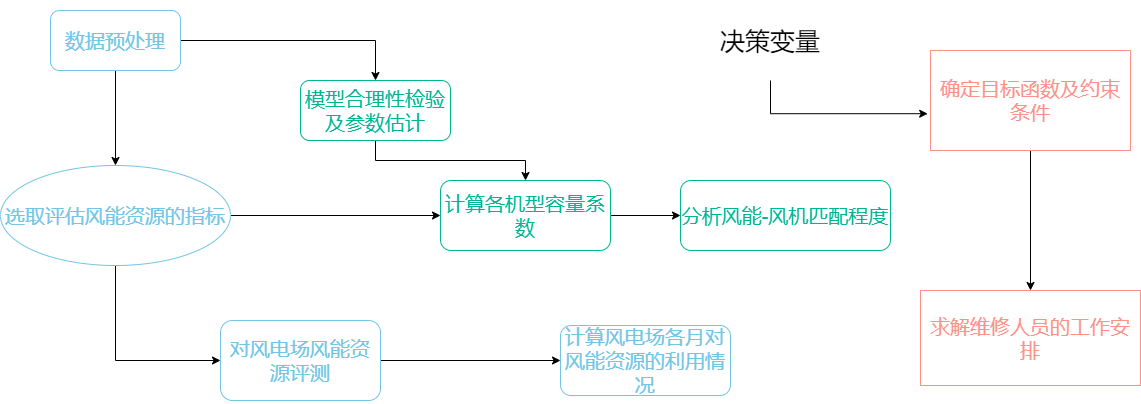
\includegraphics[width=1.\textwidth]{fig11.png}
		\caption{流程图}
		\label{fig:flow}
	\end{figure}\par
	\section{模型的建立与求解}
		\subsection{问题一:风能资源及其利用情况评估模型}
		风能资源及其利用情况的评估对风电场的运行与发展有着深远影响,不仅有助于已建成的风电场明晰自身情况并寻求改进方向以提高经济收益,同时对新风电场的选址与建设提供了指导性建议。
		\subsubsection{模型建立}
		对风能资源详细的评估能了解当地风能资源情况,有利于未来风电场的设计选择。\par
		本文从以下几个方面评估风能资源:\par
		
		\textbf{平均风速}:能清晰表示所在地风能资源状况的参数。\par
		为了更好的显示风能资源状况优劣,根据附件一给出的2015年此风电场风速数据,本文提取出此风电厂每月整点时刻平均风速计算平均值得到\textbf{月平均风速日变化值},除此之外,计算出2015年此风电厂全年整点时刻平均风速得到\textbf{年平均风速日变化值},同时,计算出全年12个月各自的平均风速得到\textbf{平均风速年变化值}。最后,由于年平均风速越大意味着该地风能资源状况较好,且此参数最能显示风能资源的优劣\supercite{风能资源评估和机组选型在风电场选址中的应用},所以我们求出2015年内该风电场风速平均值即\textbf{年平均风速值}。\par
		

		\textbf{有效小时占比}:又称风能可利用时间占比,代表测量时间内风速位于有效风速区间的累计小时数在所有小时数中的比例。有效小时占比是评价某一地区风能资源情况的重要参数,有效小时占比越大意味着风能资源越好。\par
		我们间隔1m/s取风速区间,统计2015年此风电厂各区间风速出现次数,得到\textbf{全年风速频数分布值},同时,根据我国风能区域等级划分标准,有效风速范围为3m/s——25m/s,于是我们观察全年风速频数分布,考虑风速位于3m/s——25m/s中的小时数比例评估风能资源。同时也可根据数据进行合理性检验中的范围检验(要求每小时平均风速小于等于40m/s)\supercite{风电场风能资源评估方法}
		
		\textbf{风功率密度}:气流在单位时间内垂直通过单位截面积的风能。\par
		风功率密度是衡量某一地区风能资源的综合指标,评价风能开发潜力的重要参数,同时也可以在一定程度上反映风能利用率。\par
		风功率密度计算公式为(1)、平均风功率密度$\overline{D}$计算公式为(2):
		\begin{gather}
			D_i=\frac{1}{2}\rho {v_i}^3\\
			\overline{D}=\frac{1}{n}\sum_{i=1}^{n}D_i\\
			n-\text{设定时段内的记录数} \notag \\
			\rho-\text{空气密度,单位为:}kg/m^3 \notag \\
			v^3-\text{第i次记录的平均风速的三次幂}\notag
		\end{gather}\par
		对于空气密度$\rho$,由模型的假设,设风电场空气密度为1.205$kg/m^3$。\par
		结合公式(1)、(2),利用年平均风速日变化值可直接求得该地区2015年的\textbf{年风功率密度日变化值}。另外,计算另一重要指标年(或)月平均风功率密度时,我们考虑到不可用年(或月)平均风速计
		算年(或月)平均风功率密度\supercite{风电场风能资源评估方法},于是我们提取出每小时平均风速来计算每小时平均风功率密度,得到2015年该地区每月逐小时风功率密度的平均值即\textbf{月平均风功率密度值},同时计算出了2015年该地区全年逐小时风功率密度的平均值即\textbf{年平均风功率密度值}。\par
		
		同时,本文通过以下参数评估风能资源利用状况:\par
		\textbf{风-面利用系数}:风电机从风能中捕获的能量多少可以用风能利用系数$C_p$来表示\supercite{风能资源评估和机组选型在风电场选址中的应用},$C_p$的具体表达式如下:\par
		\begin{gather}
			C_p=\frac{P}{\frac{1}{2}\rho v^3S}\\
			P-\text{风电机实际输出功率,单位为W}\notag\\
			S-\text{风轮的扫风面积,单位为$m^2$}\notag
		\end{gather}\par
		由于不知道风轮的扫风面积,于是我们假设出风-面利用系数$C_S$,具体表达式如下:
		\begin{gather}
			C_S=\frac{2P}{\rho v^3}
		\end{gather}\par
		我们通过月平均风速、附件一中的风电机实际输出功率情况计算出的月平均实际输出功率,可以计算出2015年12个月风-面利用系数,我们在比较各月风能资源利用情况时,由于扫风面积不影响比较结果,不妨假设风轮扫面的半径为55m,计算出各月风能利用系数,同时,为了对2015年全年风能资源利用情况进行一个大概评估,计算出全年风能利用系数。最后通过贝兹定律\supercite{FengNeng}评估风能资源利用状况。
		
		
		
		\subsubsection{模型求解}
		通过Matlab计算出月风速日变化值并且通过Python绘图,将12个月按季度分成四张图,如图2:
		\begin{figure}[!htbp]
			\centering
			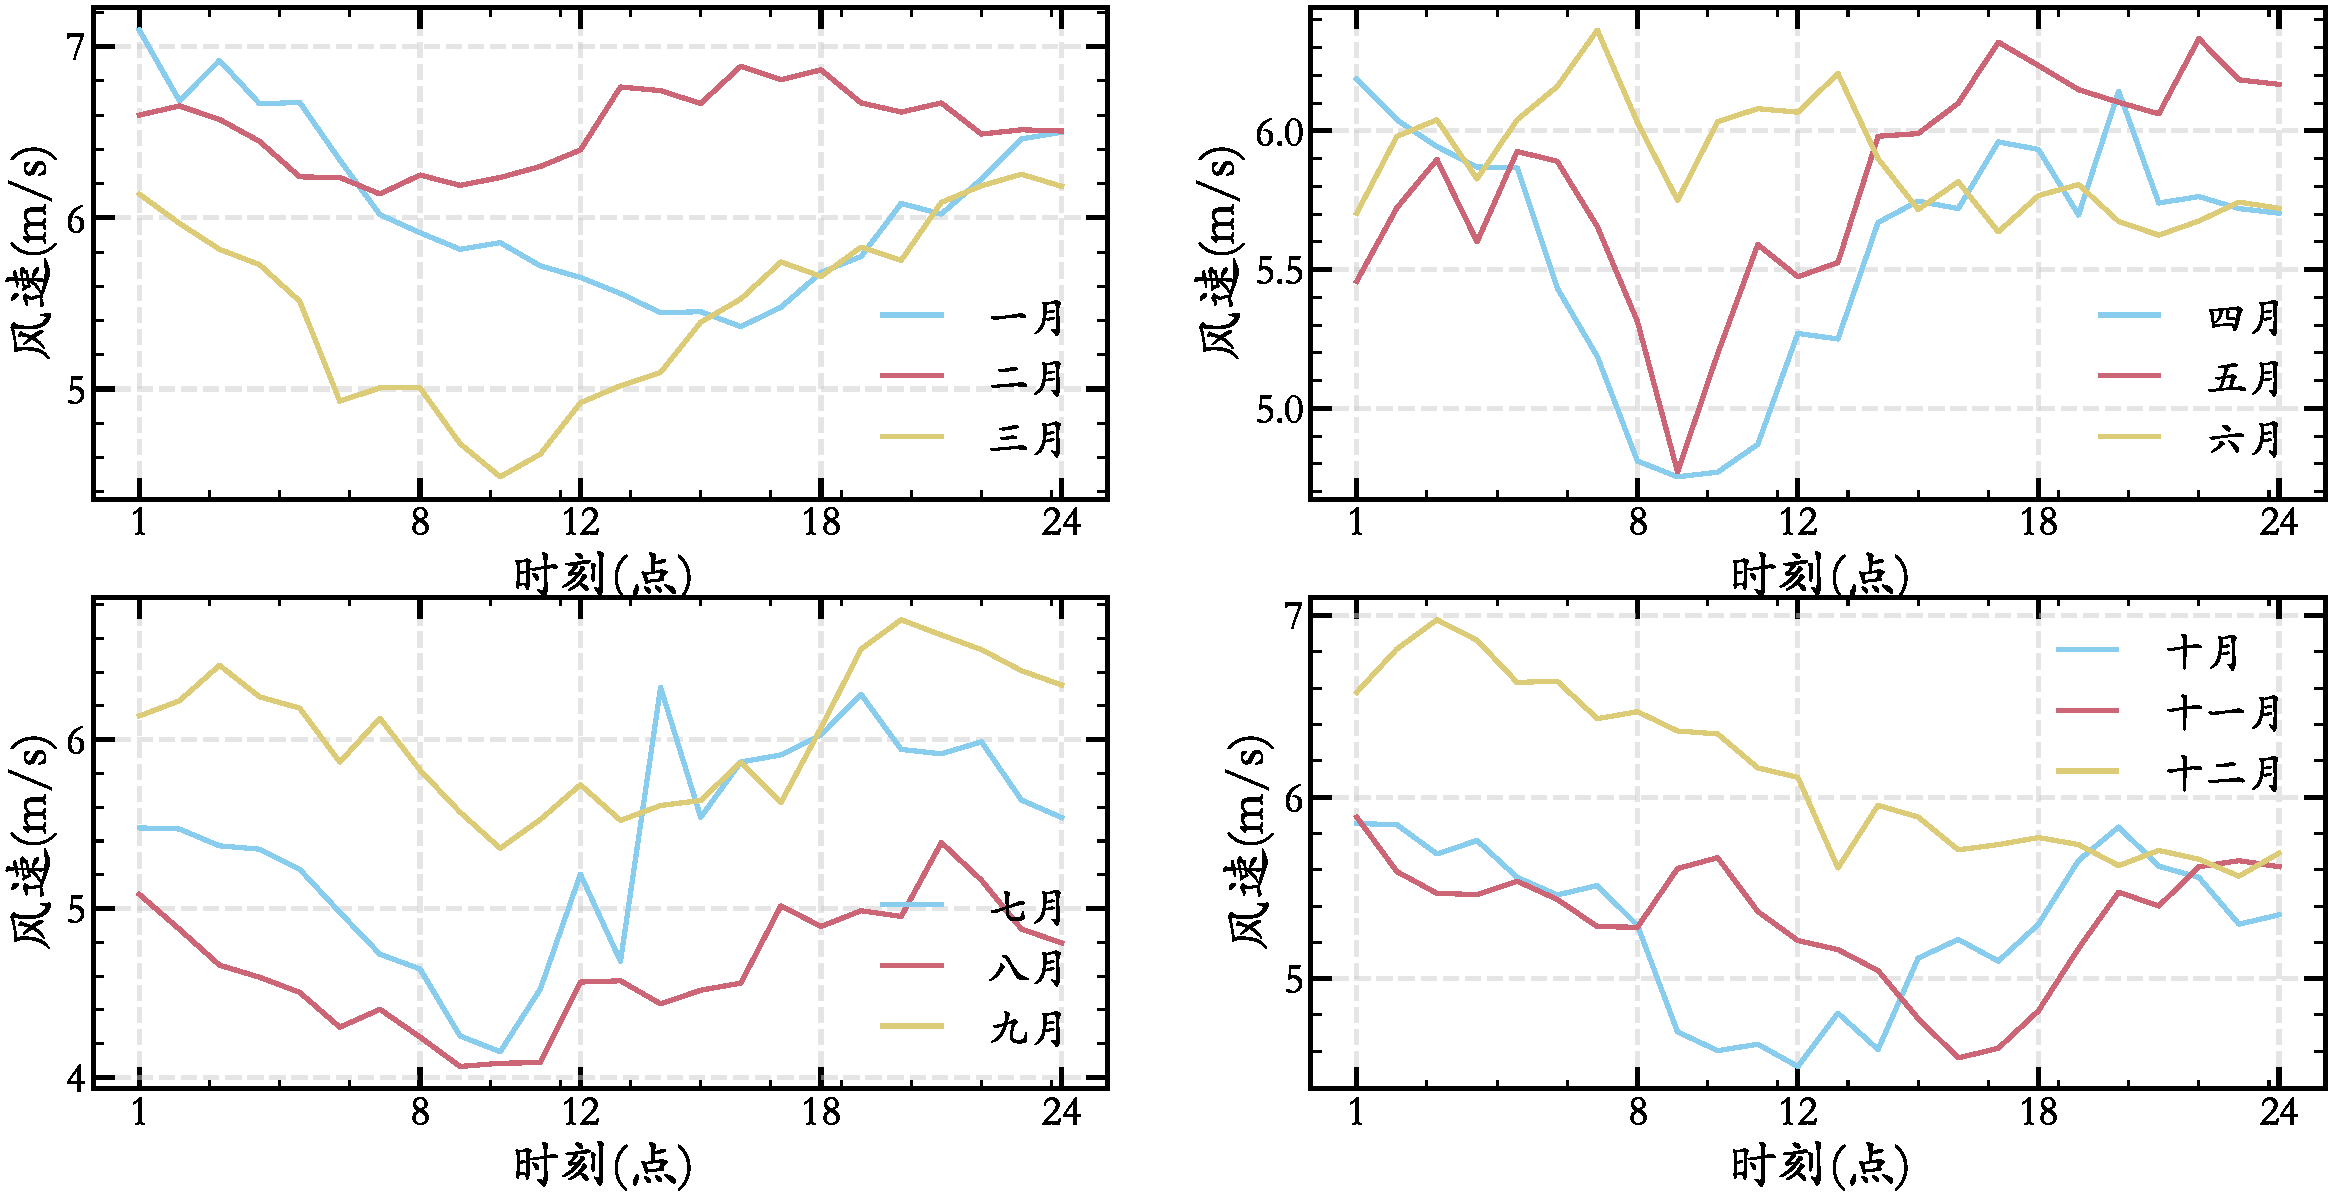
\includegraphics[width=1.\textwidth]{fig1}
			\caption{月风速日变化图}
			\label{fig:month_day}
		\end{figure}\par
		通过Matlab计算出年风速日变化值和年风功率日变化值,通过Python绘图,将两值绘制在同一张图上,如图3:
		\begin{figure}[!htbp]
			\centering
			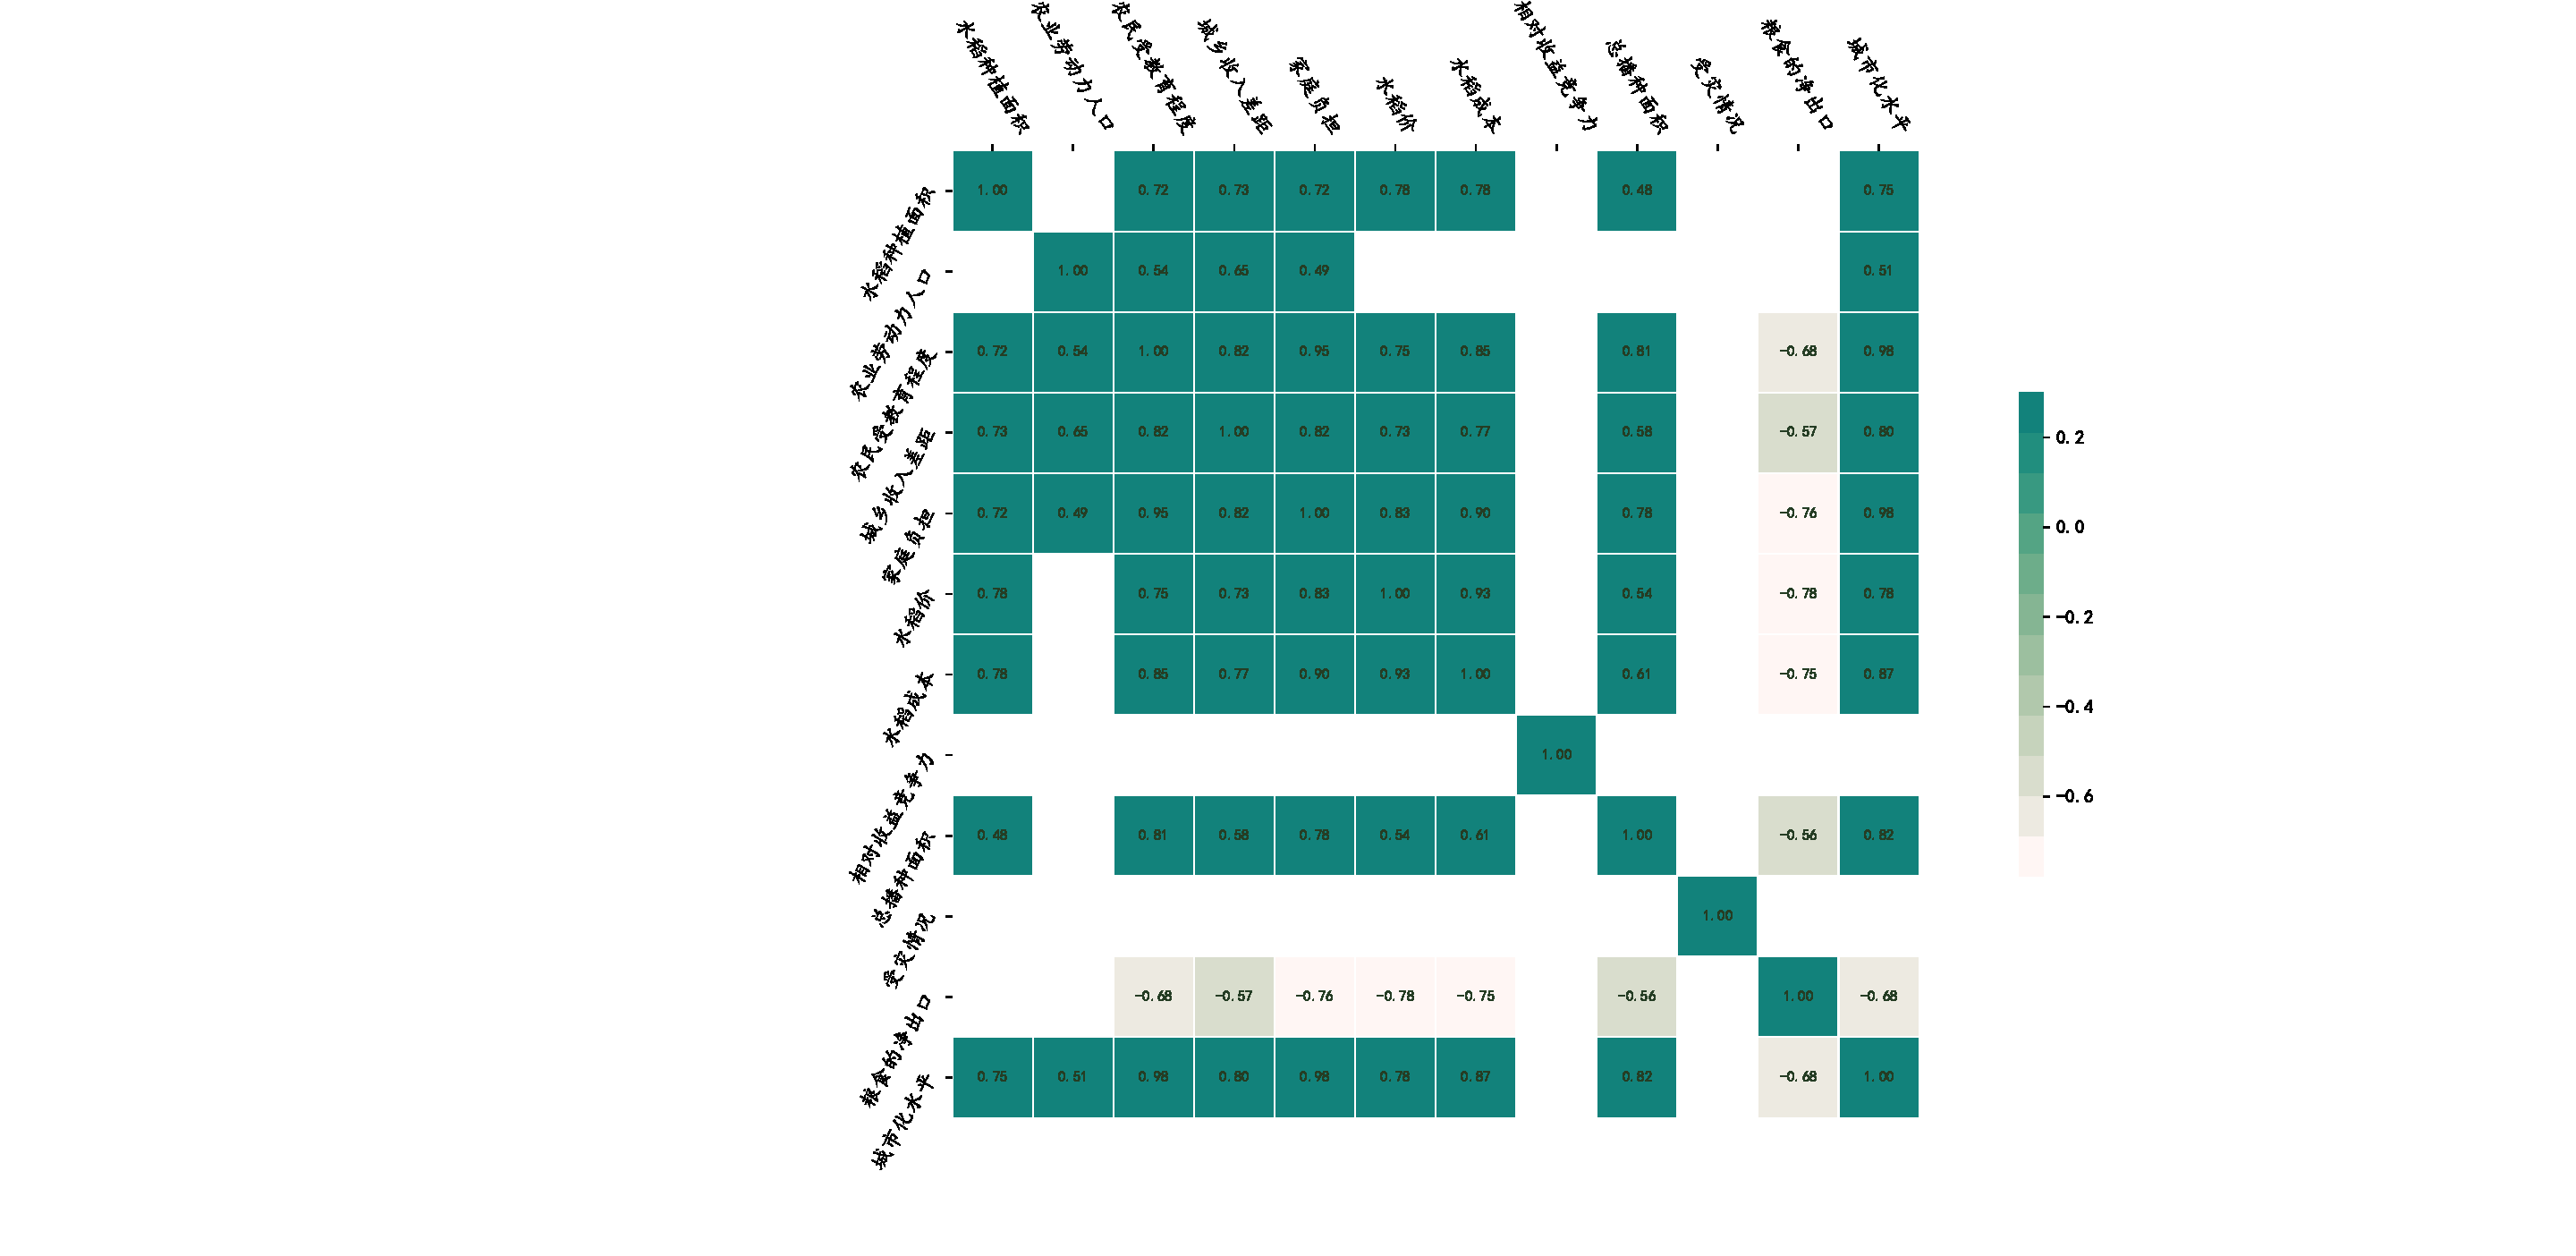
\includegraphics[width=0.9\textwidth]{fig2}
			\caption{年风速(风功率密度)日变化图}
			\label{fig:year_day}
		\end{figure}\par
		由图2和图3可以看出,从月和年的角度观察,风速每日九至十点时平均风速及平均风功率密度较低。\par
		通过Matlab计算出风速、风功率密度年变化值并通过Python将其绘制在同一张图上,如图4:
		\begin{figure}[!htbp]
			\centering
			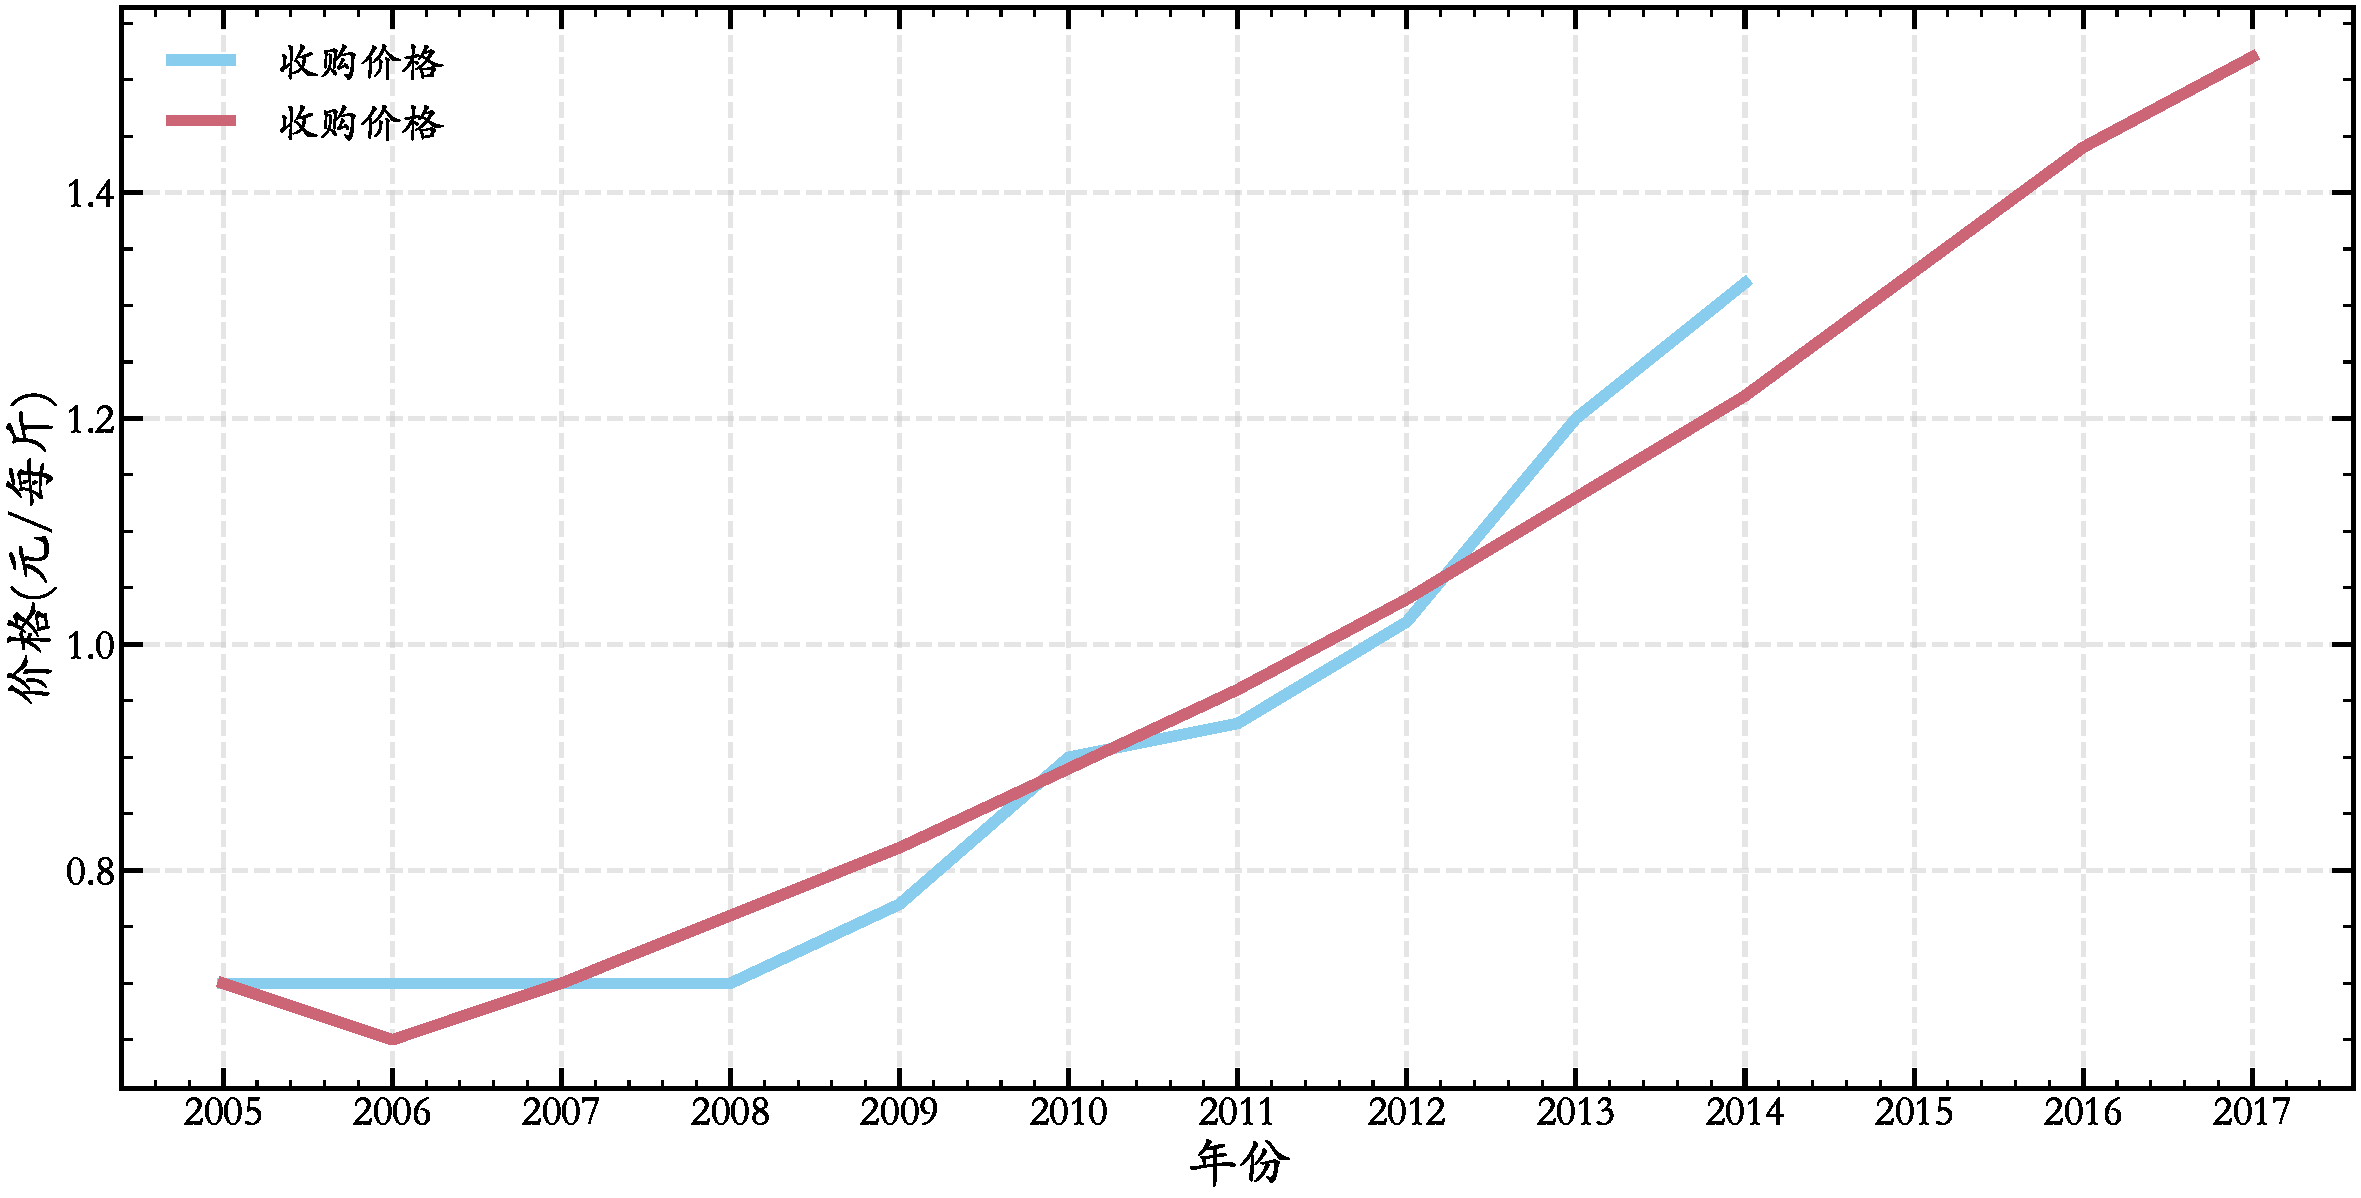
\includegraphics[width=1.\textwidth]{fig3}
			\caption{风速、风功率密度年变化图}
			\label{fig:year}
		\end{figure}\par
		通过Matlab计算出全年风速频数分布并通过Python绘制出分布直方图,并在图中划分出有效风速范围并指出该地区全年有效小时数所占比例为$84\%$,说明风能资源状况较好,同时所有平均风速皆小于40m/s,通过合理性检验。如图5:
		\begin{figure}[!htbp]
			\centering
			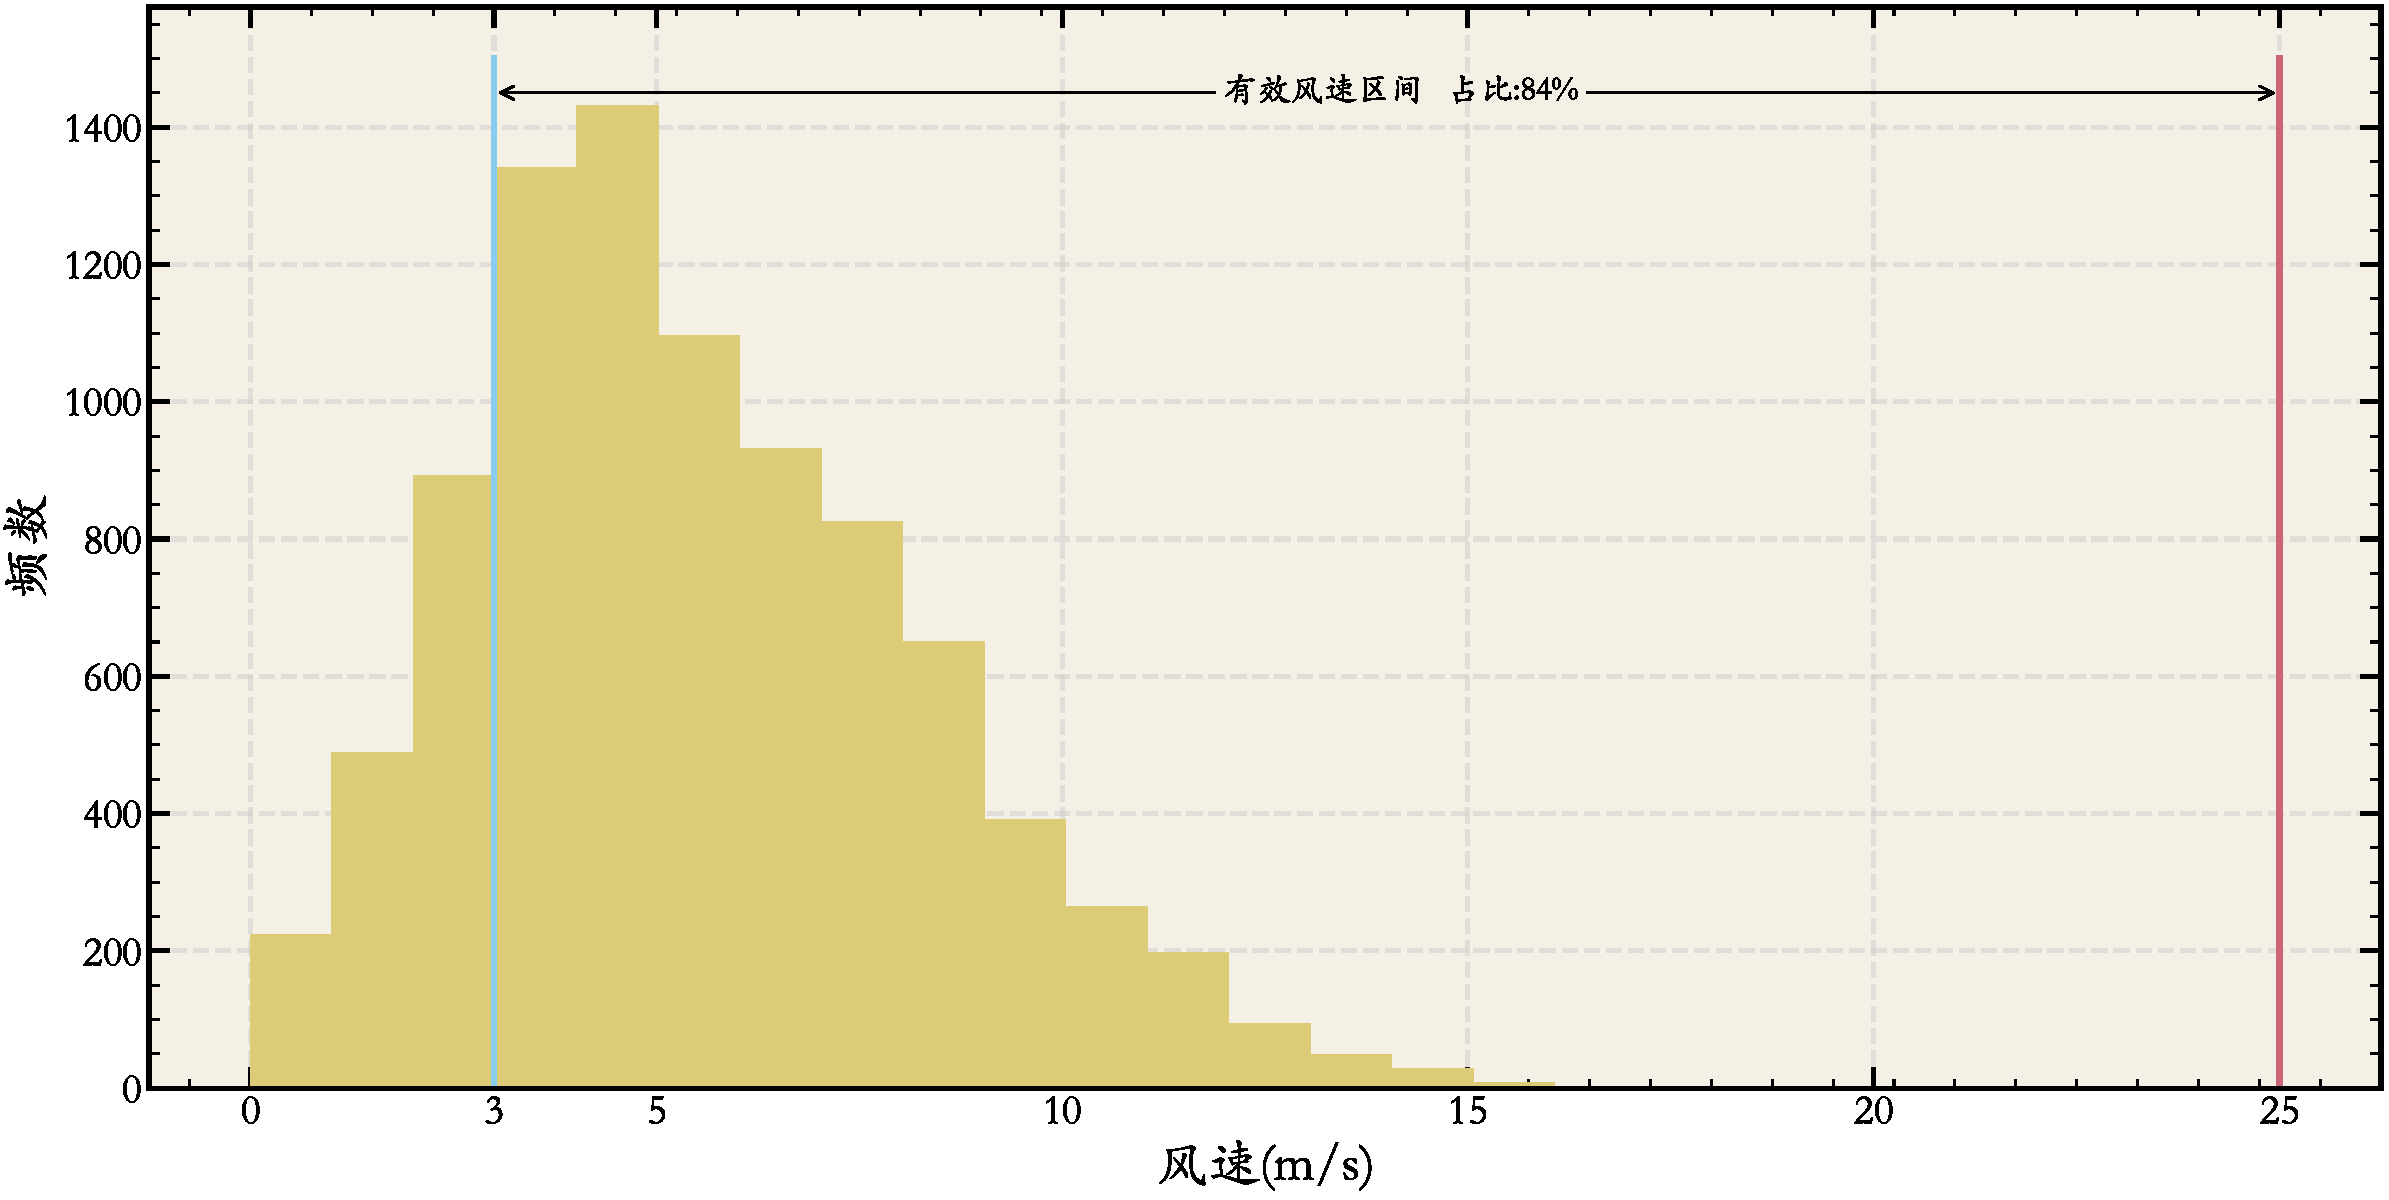
\includegraphics[width=1\textwidth]{fig4}
			\caption{全年风速频数分布直方图}
			\label{fig:fenbu}
		\end{figure}\par
		通过Matlab计算出年平均风速为$5.6756m/s$、年平均风功率密度$157.7927W/m^2$,通过与表2\supercite{风能资源评估和机组选型在风电场选址中的应用}比对:
		\begin{table}[!htbp]
			\caption{10m高度风功率密度等级}\label{tab:001} \centering
			\begin{tabular}{cccc}
				\toprule[1.5pt]
				风功率密度等级 & 风功率密度$(W/M^2)$ & 年平均风速参考值 & 应用电网发电\\
				\midrule[1pt]
				1 & <100 & 4.4 & 较差 \\
				2 & 100-150 & 5.1 & 一般 \\
				3 & 150-200 & 5.6 & 较好 \\
				4 & 200-250 & 6.0 & 好 \\
				5 & 250-300 & 6.4 & 很好 \\
				6 & 300-400 & 7.0 & 很好 \\
				7 & 400-1000 & 9.4 & 很好 \\
				\bottomrule[1.5pt]
			\end{tabular}
		\end{table}\par
		由表2,对比10m高度风功率密度等级,由计算出的年平均风速和年平均风功率密度可得该地风能资源状况较好。\par
		通过Matlab计算出当风轮扫面半径为55m时各月风能利用系数,通过Python绘图,如图5:
		\begin{figure}[!h]
			\centering
			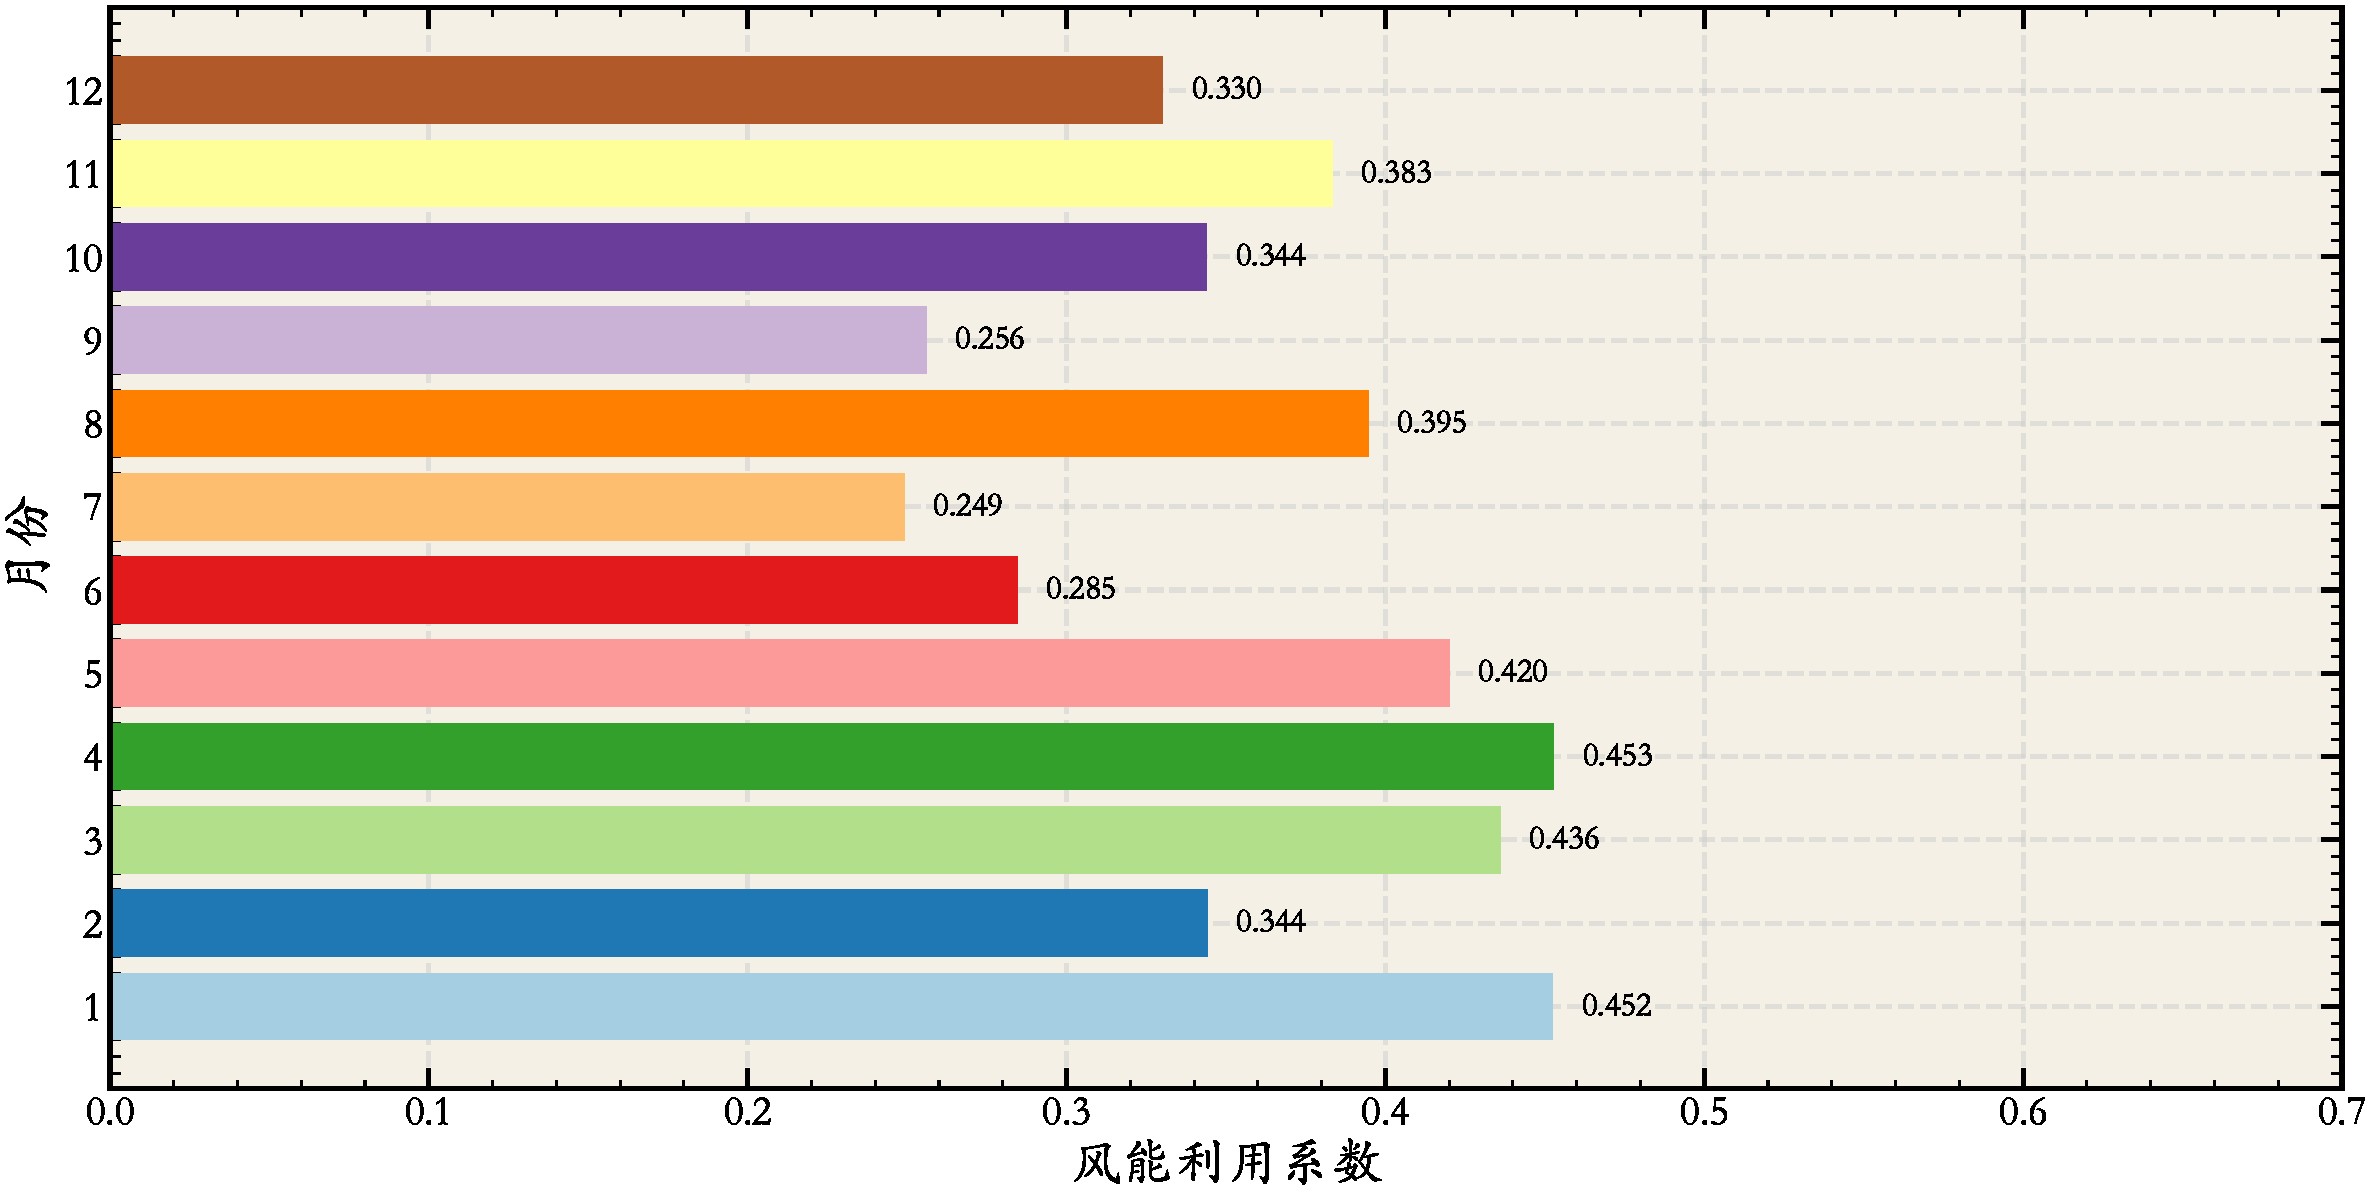
\includegraphics[width=1.\textwidth]{fig5}
			\caption{各月风能利用系数}
			\label{fig:liyong}
		\end{figure}\par		
		通过Matlab计算出当风轮面积为55m时年风能利用系数为0.369,低于贝兹极限0.596,是合理的且说明该风电场风能利用情况较好。
		\subsection{问题二:风能-风机匹配评估模型}
		风力机组的评价,除了与风电机组本身的型号及其参数(切入风速、切出风速、额定风速、额定功率等)有关,也取决于风力机组与所在地风能资源的匹配程度,本文利用容量系数最优方法判断新机型是否比现有机型更适合。
		\subsubsection{模型建立}
		\begin{figure}[!h]
			\centering
			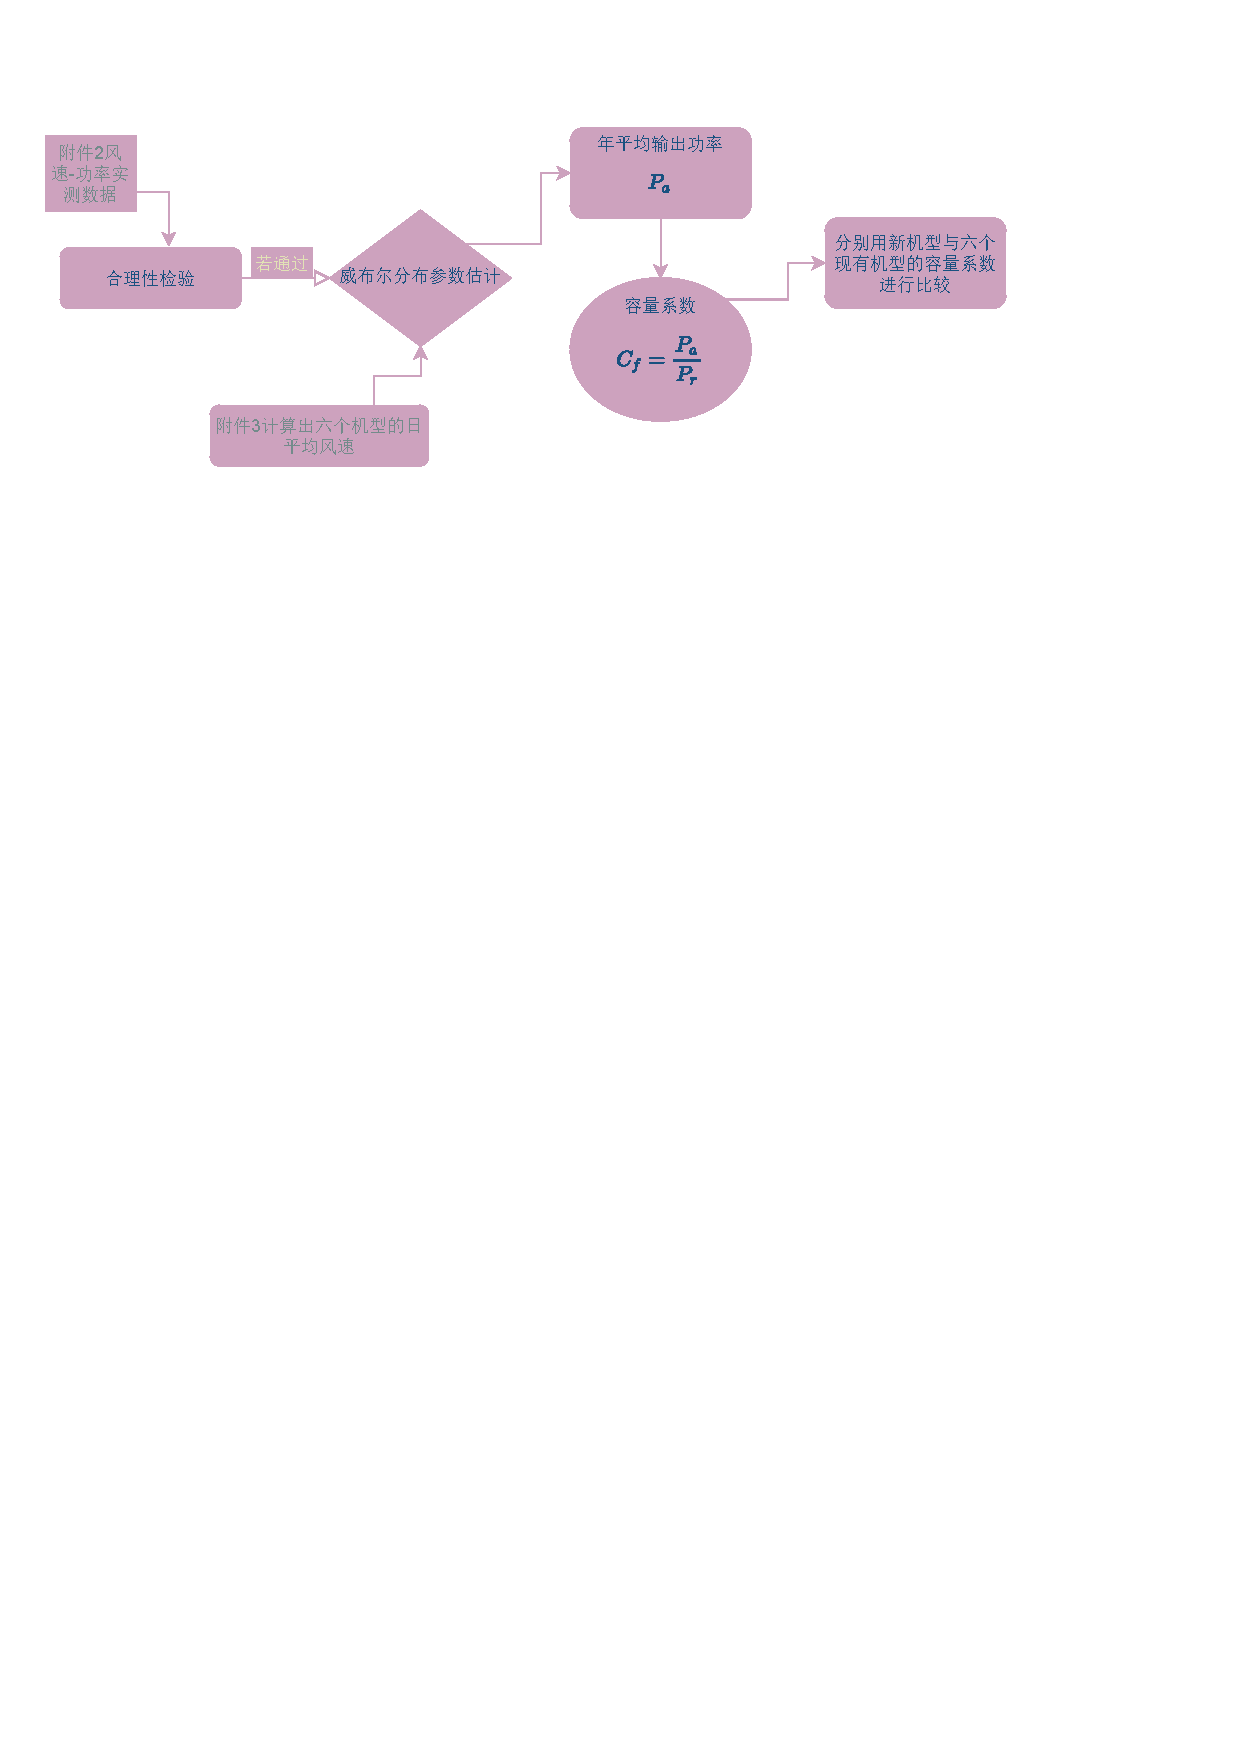
\includegraphics[width=1.\textwidth]{fig6}
			\caption{模型二流程图}
			\label{fig:model2}
		\end{figure}\par
		根据附件二、附件三、附件四,所能利用的数据仅有原有机型所在地的风速信息、原有机型和新机型的型号及部分参数。我们想要更加严谨的评估风能资源与风机匹配程度即避免假设参数,查阅资料后发现容量系数这一参数能够符合我们的要求,此参数式风电场建设中风电机组选型的重要参数。容量系数仅涉及某地风能情况,根据风速与输出功率的函数以及风机本身参数即可计算,我们假设新机型接受各地原有机型处的风能资源,逐次比较容量系数即可完成评估\par
		$Step1\quad\textbf{合理性检验:}$风力机的输出功率可以由风速来表示,并且有风力机的功率输出特性曲线,表达式如下\supercite{风能资源评估和机组选型在风电场选址中的应用}:\par
		\begin{gather}
		P(v) =
		\begin{cases}
			0 &  0\leq v<v_i\\
			\eta(v) P_r &   v_i\leq v<v_r\\
			P_r & v_r\leq v\leq v_c\\
			0 & v>v_c
		\end{cases}\\
		v_i-\text{风电机切入风速}\notag\\
		v_r-\text{风电机额定风速}\notag\\
		v_c-\text{风电机切出风速}\notag\\
		P_r-\text{风力发电机额定输出功率}\notag\\
		\eta(v)-\text{切入风速和额定风速之间,风电机输出功率随风速变化的函数关系}\notag
		\end{gather}\par
		上述$\eta(v)$输出特性理论上可以表示成三次函数\supercite{风电场运行状况分析及优化},于是我们利用附件三两种型号风机的风速-功率实测数据,拟合三次函数$\eta(v)=a+bx^3$。\par
		$Step2\quad \textbf{威布尔函数参数估计:}$为了求出容量系数,我们利用附件二,首先对原有风电机组中的六个机型利用最小二乘法分别进行威布尔参数估计(每个机型所处位置不同,风能资源不同):
		\begin{itemize}
			\item 分别计算出六个机型风电机的日平均风速,得到各自日平均风速涵盖范围,取1m/s为步长划分成n个风速段:$(0\sim v_i),i=1,\dots,n$。
			\item 统计六个机型风电机每个风速段日平均风速出现的频率$p_i,i=1,\dots,n$。
			\item 做如下变换:
			\begin{gather*}
				x_i=lnv_i\\
				y_i=ln[-ln(1-p_i)]\\
				\overline{x}=\frac{1}{n}\sum_{i=1}^{n}x_i\\
				\overline{y}=\frac{1}{n}\sum_{i=1}^{n}y_i\\
				k=\frac{\sum_{i=1}^{n}\left[\left(x_{i}-\bar{x}\right)\left(y_{i}-\bar{y}\right)\right]}{\sum_{i=1}^{n}\left(x_{i}-\bar{x}\right)^{2}} \\
				c=\exp \left[-\left(\frac{\bar{y}}{k}-\bar{x}\right)\right]
			\end{gather*}
		得到威布尔分布重要参数k、c。
		\end{itemize}\par
		$Step3\quad \textbf{计算年平均输出功率:}$得到双参数威布尔分布函数\supercite{威布尔分布}如下:
		\begin{gather}
			P_{w}(v)=
			 \begin{cases}
			\frac{k}{c}\left(\frac{v}{c}\right)^{k-1} \exp \left[-\left(\frac{v}{c}\right)^{k}\right]&x\geq0\\
			0 &  x<0 
			\end{cases}
		\end{gather}\par
		由风力机功率输出特性表达式及威布尔分布函数(6)可计算出风电机年平均输出功率:
		\begin{gather}
			P_{a}=\frac{P_{r}}{\left(v_{r}-v_{i}\right)^{3}} \int_{v_{i}}^{v_{r}}\left(v-v_{i}\right)^{3} P_{w}(v) d v+P_{r} \int_{v_{r}}^{v_{c}} P_{w}(v) d v
		\end{gather}\par
		$Step4\quad \textbf{计算容量系数:}$于是容量系数$C_f$的具体表达式\supercite{风能资源评估和机组选型在风电场选址中的应用}为:
		\begin{align}
			C_f&=\frac{P_a}{P_r}\notag\\
	           &=\frac{1}{\left(v_{r}-v_{i}\right)^{3}} \int_{v_{i}}^{v_{r}}\left(v-v_{i}\right)^{3} P_{w}(v) d v+\int_{r_{r}}^{v_{c}} P_{w}(v) d v		
		\end{align}\par
		\subsubsection{模型求解}
		利用Matlab,绘制出合理性检验的拟合函数图,如图7:
\begin{figure}[!h]
	\centering
	\begin{minipage}[c]{0.48\textwidth}
		\centering
		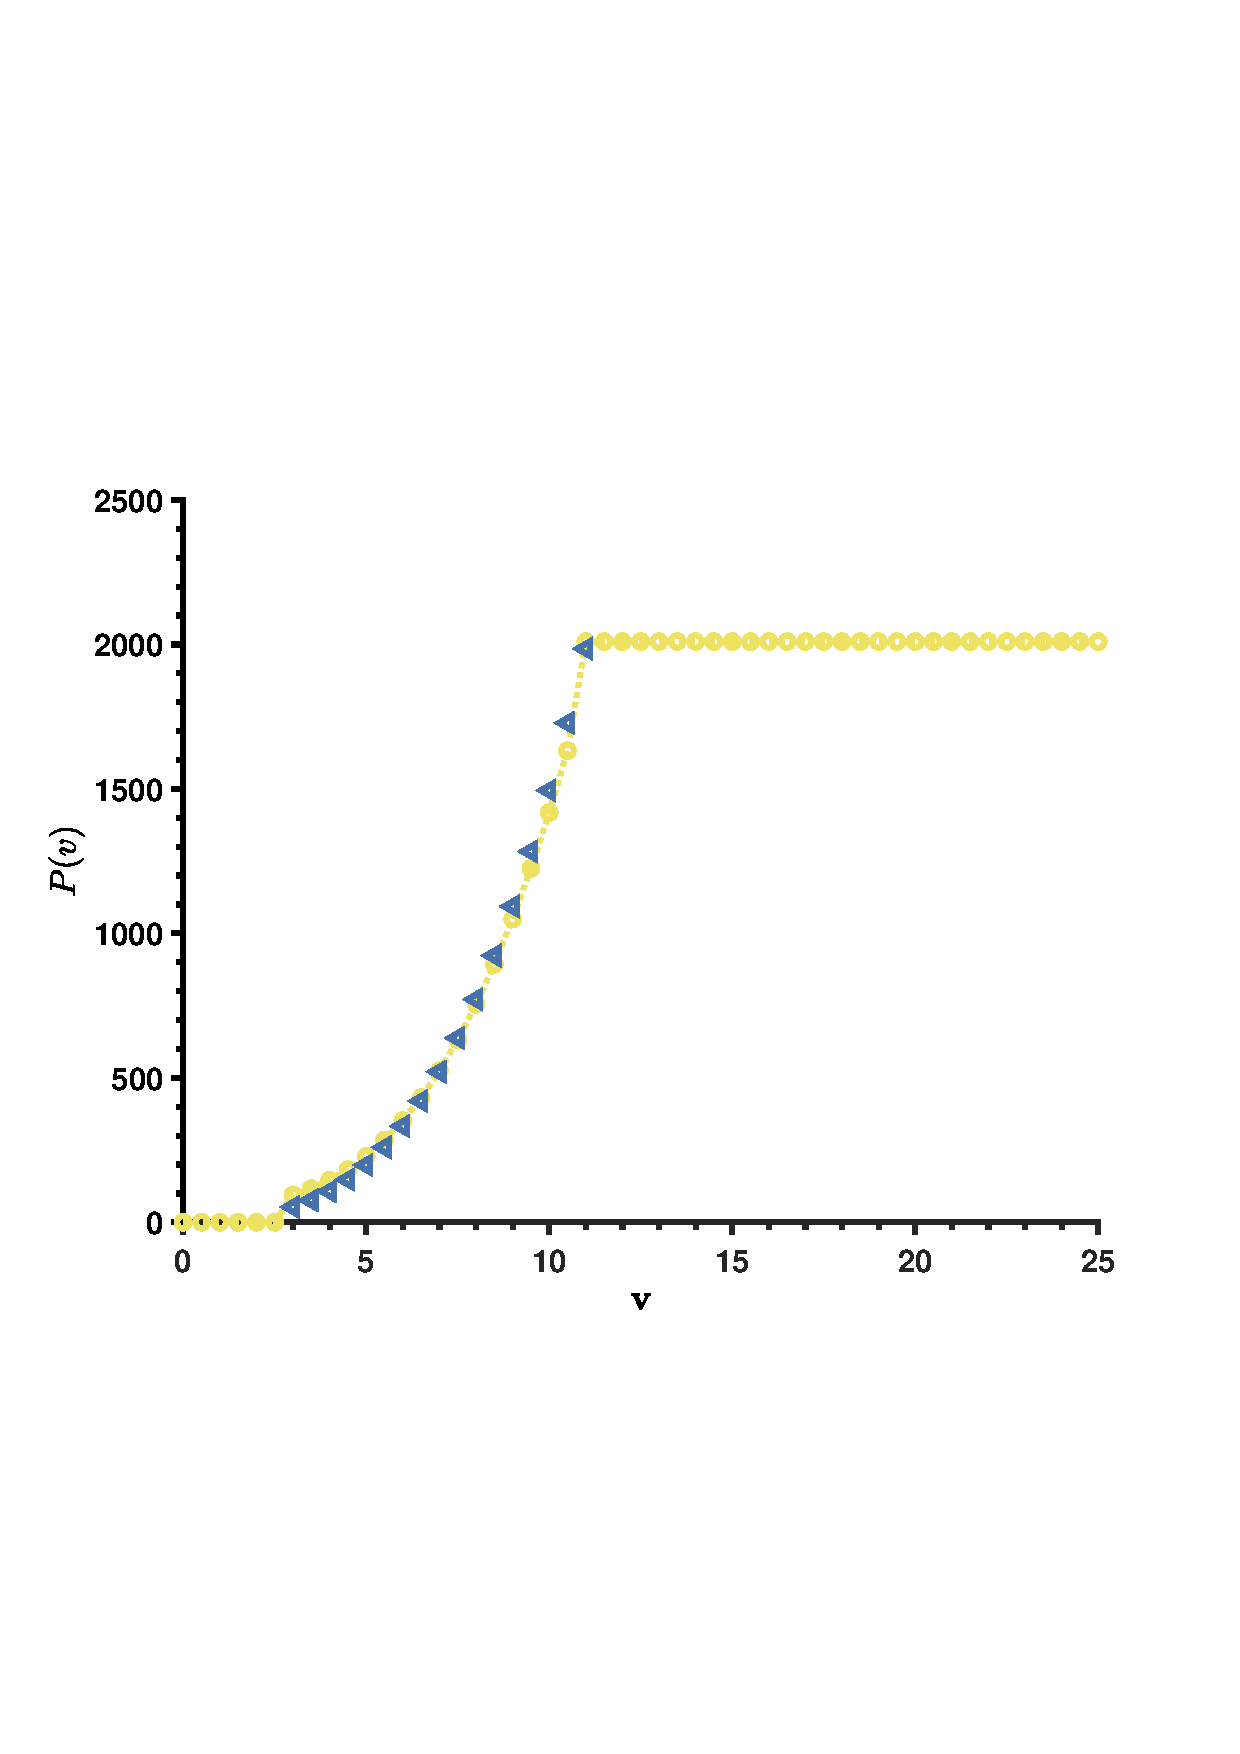
\includegraphics[width=0.95\textwidth]{fig7}
		\subcaption{机型一}
		\label{fig:sample-figure-a}
	\end{minipage}
	\begin{minipage}[c]{0.48\textwidth}
		\centering
		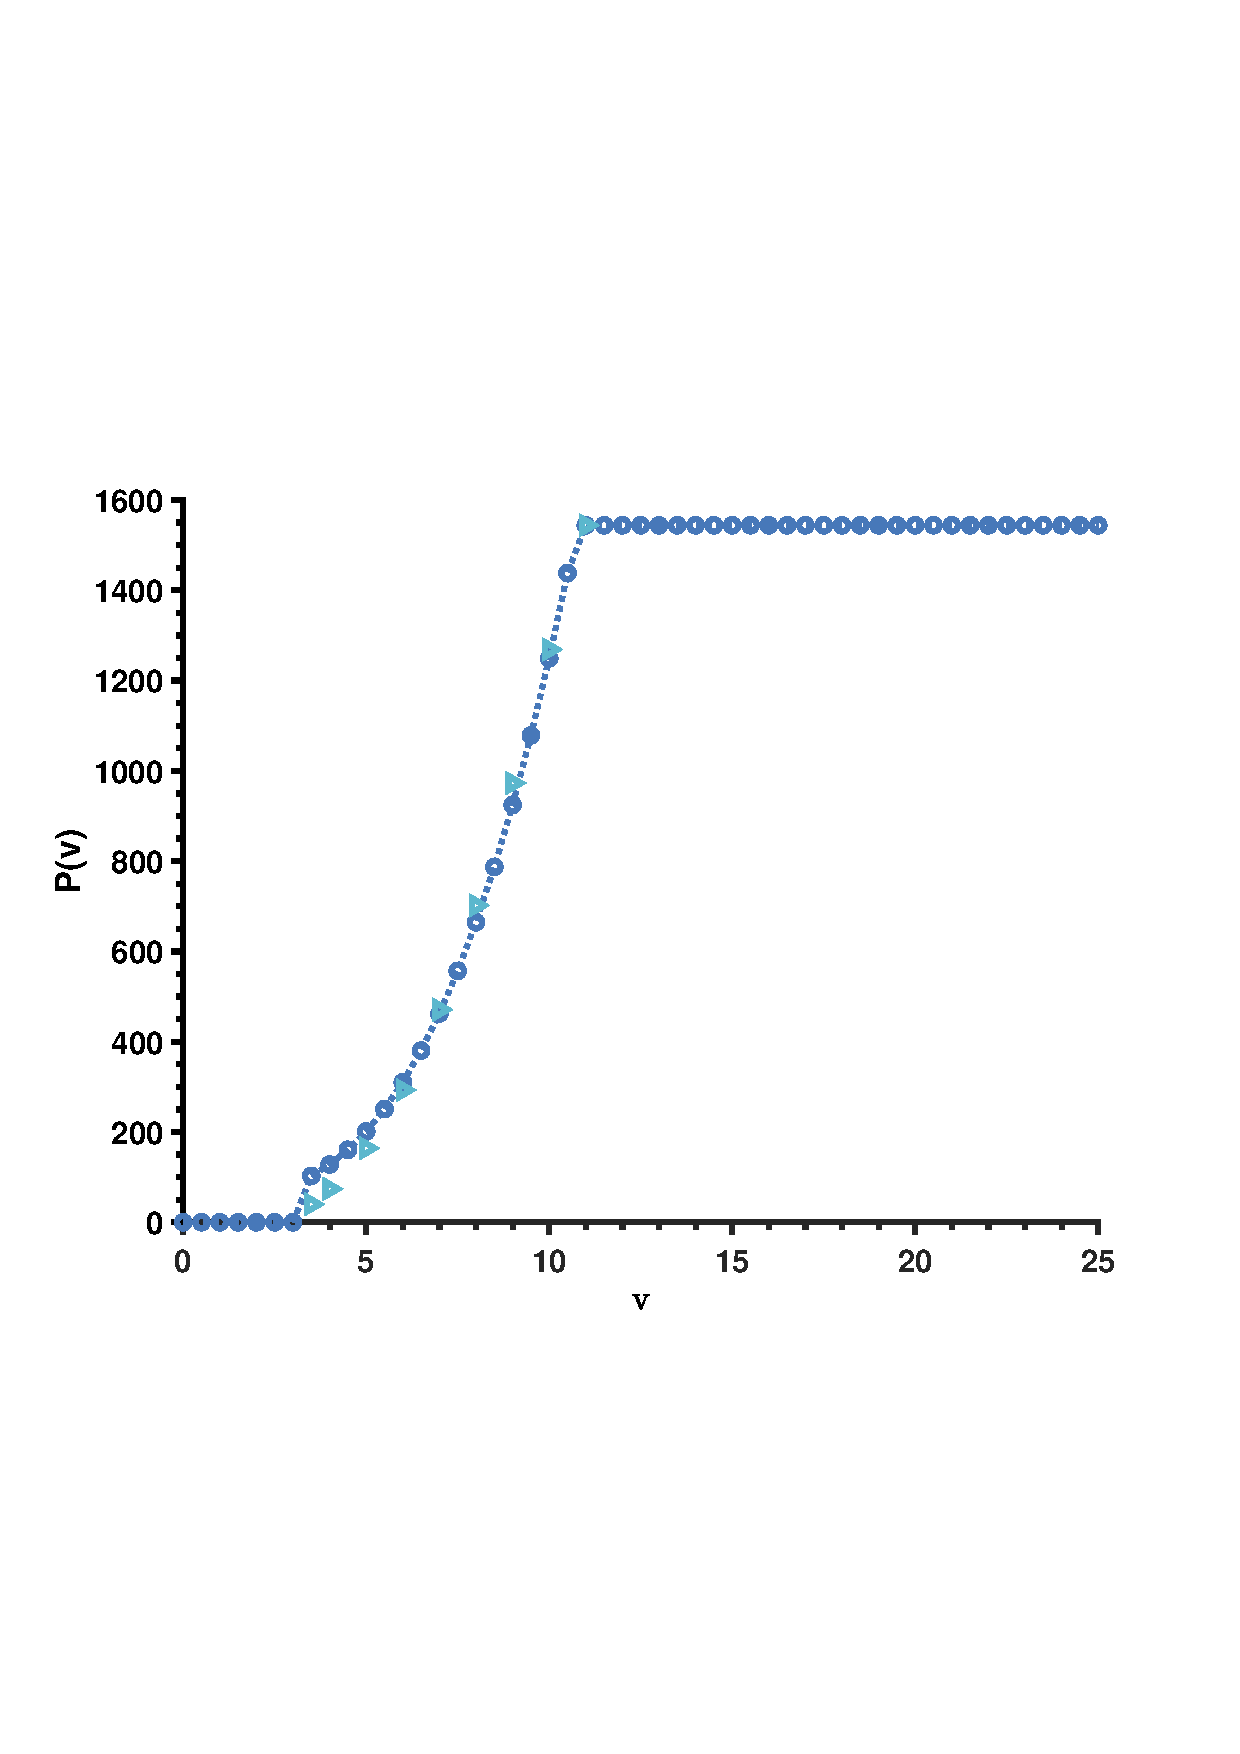
\includegraphics[width=0.95\textwidth]{fig8}
		\subcaption{机型二}
		\label{fig:sample-figure-b}
	\end{minipage}	
	\caption{风速-输出功率拟合图}
	\label{fig:sample-figure}
\end{figure}\par
		拟合优度分别为:0.9984、0.9915,说明曲线符合风力机功率输出特性即当地风力情况及两原有机型情况正常,通过合理性检验。\par
		按照模型求解中的流程,编写Matlab程序可求解出六个原有机型与新机型的容量系数,由于六个原有机型又分别属于两种机型,于是我们利用Python绘制出机型一、机型二分别与新机型的容量系数对比玫瑰图,如图8所示。
		\begin{figure}
			\centering
			\begin{minipage}[c]{0.95\textwidth}
				\centering
				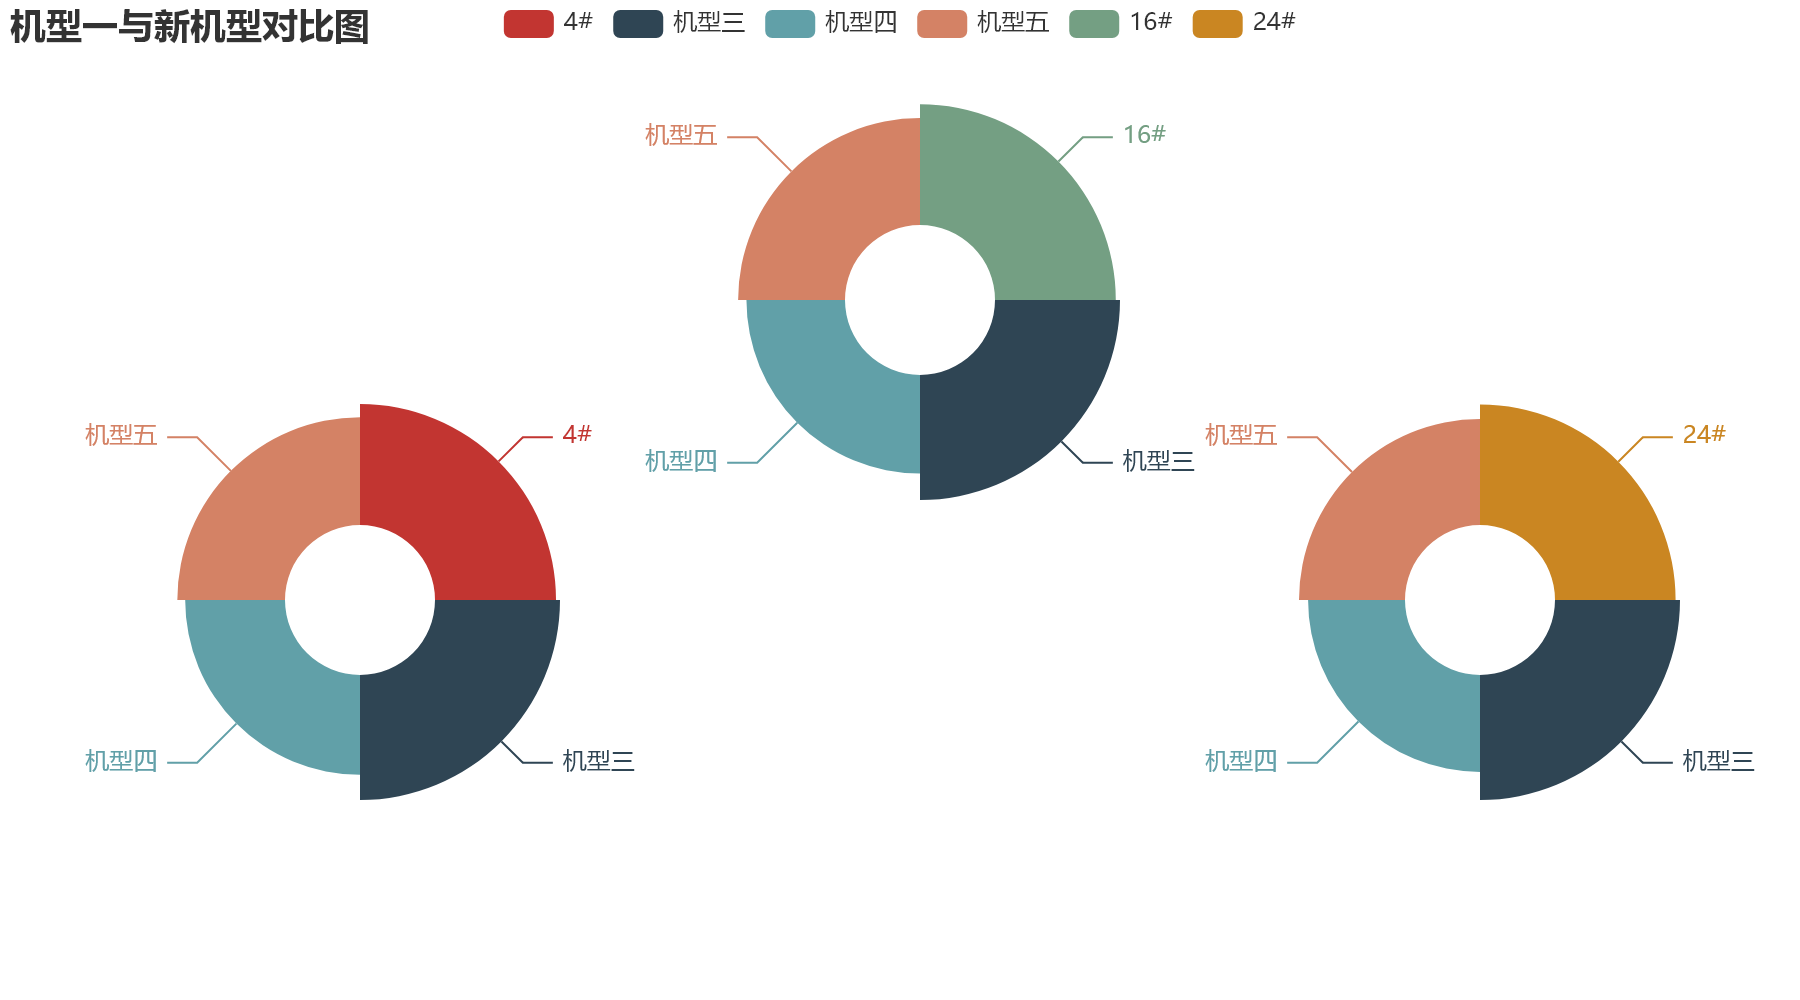
\includegraphics[width=1\textwidth]{fig9.png}
			\end{minipage}
			\begin{minipage}[c]{0.95\textwidth}
				\centering
				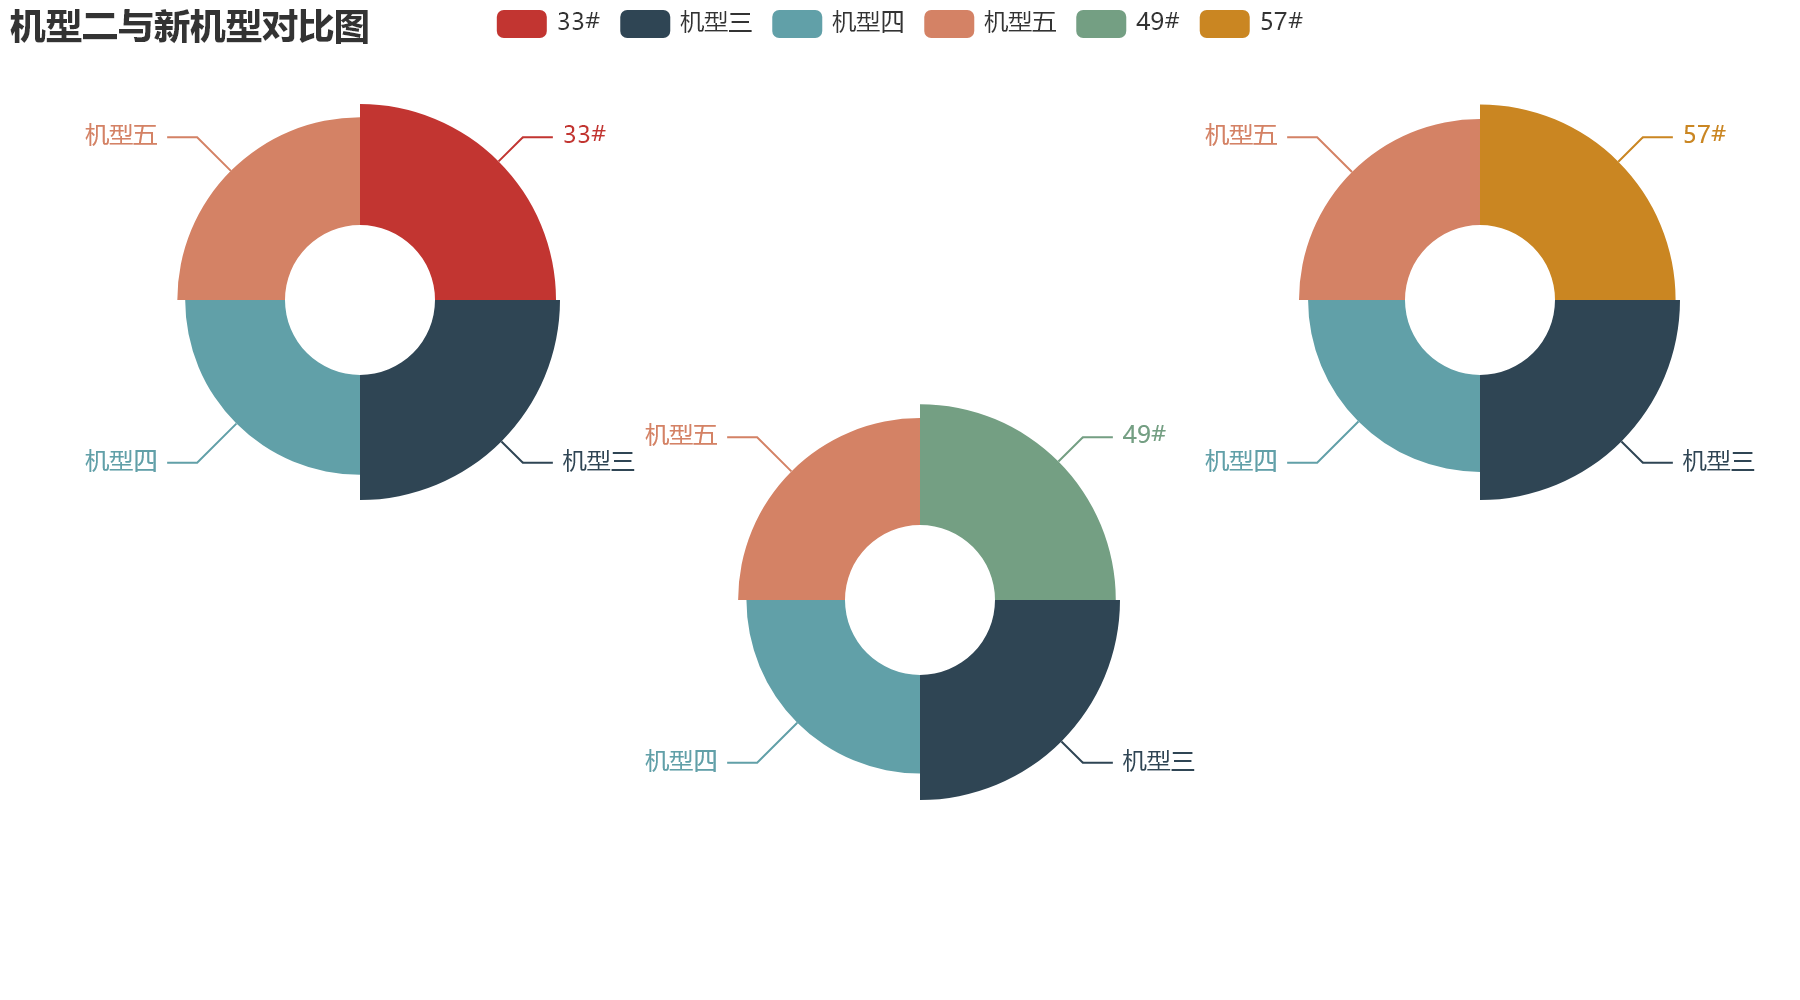
\includegraphics[width=1\textwidth]{fig10.png}
			\end{minipage}
			\caption{容量系数比较图}
		\end{figure}\par
		由图可知,与所有原有机型对比后,机型三与各地风能资源匹配程度最好,所以我们认为机型三比原有机型更为合适,而机型四与机型五相较原有机型而言,与当地风能资源匹配程度较差,即机型三、机型四并不合适。
		\subsection{问题三:风电场排班规划模型}
		对于此风电厂124台风电机以及4组维修人员,根据题意,为了使各组维修人员的工作任务相对平衡,且风电场具有良好的经济效益,124台风电机的停机维护计划方案和4组维修人员的值班(维护)安排可以使用0-1整数规划求解。
		\subsubsection{模型建立}
		设变量
		\[
		x_{it} =
		\begin{cases}
			1 &  \text{第i台风机在第t天维修}\\
			0 &  \text{第i台风机在第t天不维修}
		\end{cases}
		\]
		\[
		y_{jt}=
		\begin{cases}
			1 &  \text{第j支维修队在第t天维修} \\
			0 &  \text{第j支维修队在第t天不维修} 
		\end{cases}
		\]
		\[
		z_{jt}=
		\begin{cases}
			1 &  \text{第j支维修队在第t天值班}\\
			0 &  \text{第j支维修队在第t天不值班}
		\end{cases}
		\]\par
		其中$i=1,\dots,124$表示124台风机,$j=1,2,3,4$表示维修队,$k=1,\dots,365$表示一年天数。\par
		求解出问题一中的每日平均功率记为$P_d$,由于维修时风机停机,即这段时间内输出功率为0,这导致了发电损失。可以由下式表示由于停机维修导致的发电损失,为了使风电场具有良好的经济效益,应使其尽可能小,即将其设定为目标函数。
		\begin{gather}
		min\quad W=\sum_{i=1}^{124}\sum_{t=1}^{365}P_{j}x_{it}
		\end{gather}\par
		下面给出约束条件:\par
		为安全需求,每台风机一年需要维修两次,且每次维修两天,所以有:
		\begin{gather}
		\sum_{t=1}^{365}x_{it}=4\\
		i=1,\dots,124\notag
		\end{gather}\par
		风机在两次维修之间连续工作的时间不超过270天,即从任意某天开始,在之后的271天内(且不跨年)至少有一天在维修,所以有:
		\begin{gather}
			\sum_{t=d}^{d+270}x_{it}\geq1\\
			d=1,\dots,95\notag\\
			i=1,\dots,124\notag
		\end{gather}\par
		任意一天进行维修工作的组数等于该天维修的风机数量,所以有:
		\begin{gather}
			\sum_{i=1}^{124}x_{it}=\sum_{j=1}^{4}y_{jt}\\
			t=1,\dots,365\notag
		\end{gather}\par
		若某一组当天进行维修工作,则值班的任务不能由该组完成,所以有:
		\begin{gather}
			y_{jt}+z_{jt}\leq 1\\
			j=1,2,3,4\notag\\
			t=1,\dots,365\notag
		\end{gather}\par
		由于四组维修人员每天需要一组值班,故一天内至多三组进行维修工作,所以有:
		\begin{gather}
			\sum_{j=1}^{4}y_{jt}\leq 3\\
			t=1,\dots,365\notag
		\end{gather}\par
		每组维修人员连续工作时间(值班或维护)不超过6天,所以有:
		\begin{gather}
			\sum_{t=f}^{f+6}(y_{jt}+z_{jt})\leq 6\\
			f=1,\dots,359\notag\\
			j=1,2,3,4\notag
		\end{gather}\par
		每天需要且仅需要一组值班人员,所以有
		\begin{gather}
			\sum_{j=1}^{4}z_{jt}= 1\\
			t=1,\dots,365\notag
		\end{gather}\par
		每次维护需一组维修人员连续工作2天,可以通过任意一天的前后连续三天的关系进行约束,有:
		\begin{gather}
			\sum_{t=k-1}^{k+1}x_{it}\geq 2x_{ik}\\
			i=1,\dots,124\notag\\
			k=2,\dots,364\notag
		\end{gather}\par
		为使组与组之间的工作量均衡,即每组工作时长相等,所以有:
		\begin{gather}
			\sum_{t=1}^{365}(y_{jt}+z_{jt})=\sum_{t=1}^{365}(y_{j+1,t}+z_{j+1,t})\\
			j=1,2,3,4\notag
		\end{gather}\par
		综上,由目标函数(9)以及约束条件(10)-(18)可构建0-1整数规划数学模型。
		\subsubsection{模型求解}
		利用Matlab计算可以求出发电量损失为$6.24×10^{12}J$,且维修队全年工作天数为231天。
		同时我们发现若使式(18)的约束为每组工作时长之间差额不超过5天,则维修队全年工作天数分别为:217、214、221、220天,同时发电损失为$6.88×10^{12}J$。
		
		
		
		
		\section{模型的检验}
		本文在问题二计算容量系数时,假设空气密度为$1.205kg/m$,风轮的扫风半径为$55m$,我们利用Matlab对两参数进行了灵敏度分析,结果如下:\par
		当空气密度变化$10\%$时,年容量系数变化$5\%$左右,当扫风半径改变$10\%$时,年容量系数变化$10\%$左右,可以见得,容量系数对空气密度以及风轮扫风面积不敏感,即模型的稳定性较高。
	
	
	
	
	
		\section{模型的评价及推广}
		\subsection{模型评价}
		\subsubsection{优点:}\par
		1.在处理数据时进行了数据的合理性检验,提高了数据的可靠性和科学性。\par
		2.灵活运用matlab对数据进行处理运算,Python进行数据的可视化。\par
		3.遵循科学严谨的原则对风能资源,风机匹配等问题进行求解。\par
		
		\subsubsection{缺点:}\par
		1.对数据的处理存在舍入误差,模型的精确度有一定降低。\par
		2.对于问题三所确定的排班方案,编程计算时时间较长
		
		
		\subsection{模型的推广}
		本文在评价风电场资源的利用所采用的方法,可以通过改变拟合的分布推广到对其他能源,如水资源、光能资源等的评价,解决诸多领域的问题。\par
		运用了整数规划的方法,具有普适性,且对于实际风电场排班方案给出了一定程度上的建议。
	
\bibliography{book.bib}
\newpage%附录新起一页
\begin{appendices}		
	\section{matlab 源代码}
	\begin{matlab}
	clc,clear all;
	for j=1:12
		filename=['./2015',num2str(j,'%02d'),'.xls'];
		[Type Sheet Format]=xlsfinfo(filename);
		for i=1:length(Sheet)
			data=xlsread(filename,i,'B4:K27');
			power=data(:,1:3:10);%提取每天每时刻的发电功率
			power=power(:);%将二维数组转化成一维数组
			power=rmmissing(power);%去除每个表中返回空值的数据
			day_data(i)=mean(power);
			if
				length(Sheet)<31
				for k=length(Sheet)+1:31
					day_data(k)=0;
				end
			end
		end
		day_power(:,j)=day_data;
		month_power(j)=sum(day_power(:,j))/sum(sum(day_power(:,j)~=0));
		year_power=sum(sum(day_power))/sum(sum(day_power(:,:)~=0));
	end
	disp('day_power=')
	disp(day_power)
	disp('month_power=')
	disp(month_power)
	year_power
	\end{matlab}
	\begin{matlab}
	clc,clear,prob=optimproblem;
	P=xlsread('./day_power.xls');
	P=P(:);P(P==0)=[];%P=repmat(P,1,124);P=roundn(P,0);
	x=optimvar('x',124,365,'Type','integer','LowerBound',0,'UpperBound',1);
	y=optimvar('y',4,365,'Type','integer','LowerBound',0,'UpperBound',1);
	z=optimvar('z',4,365,'Type','integer','LowerBound',0,'UpperBound',1);
	for j=1:365
		for i=1:124
			prob.Objective=sum(sum(x(:,j))*P(j));
		end
	end
	prob.Constraints.con1=sum(x,2)==4;
	prob.Constraints.con2=sum(y,1)<=3;
	prob.Constraints.con3=sum(z,1)==1;
	con4=[];
	for i=1:3
		con4=[con4;sum(y(i,:))+sum(z(i,:))==sum(y(i+1,:))+sum(z(i+1,:))];
	end
	prob.Constraints.con4=con4;
	con5=[];
	for k=1:4
		for j=1:365
			con5=[con5;y(k,j)+z(k,j)<=1];
		end
	end
	prob.Constraints.con5=con5;
	prob.Constraints.con6=sum(x,1)-sum(y,1)==0;
	con7=[];
	for i=1:124
		for t=1:95
			con7=[con7;sum(x(i,t:t+270))>=1];
		end
	end
	prob.Constraints.con7=con7;
	con8=[];
	for i=1:124
		for m=2:364
			con8=[con8;x(i,m-1)-x(i,m)+x(i,m+1)>=0];
		end
	end
	con9=[];
	for i=1:4
		for n=1:359
			con9=[con9;sum(y(i,n:n+6))+sum(z(i,n:n+6))<=6];
		end
	end
	prob.Constraints.con8=con8;
	prob.Constraints.con9=con9;
	options.MaxTime = 5e4;
	[sol,fval,flag]=solve(prob)
	\end{matlab}




	\section{python源代码}
	\begin{python}
	#encoding=gb2312
	from matplotlib import colors
	import numpy as np
	import matplotlib.pyplot as plt
	import pandas as pd
	df = pd.read_excel('table3.xls',header=None)
	df=df.values
	print(df)
	x=np.arange(1,13)
	plt.style.use('science')
	fig, ax1 = plt.subplots()
	ax2 = ax1.twinx()
	ax1.plot(x,df[0],color='#36606A',marker='o',label=r'风速(m/s)',)
	ax1.legend()
	ax2.plot(x,df[1],linewidth=3,color='#D39570',marker='*',markersize=10,label=r'风功率密度($M/W^2$)')
	ax2.legend()
	ax1.set_xlabel('月份')
	plt.show()
	\end{python}
	\begin{python}
	#encoding=gb2312
	from pyecharts import options as opts
	from pyecharts.charts import Pie
	from pyecharts.faker import Faker
	import pandas as pd
	df=pd.read_excel('table6.xlsx')
	df=df.values
	v1 = ['4#','机型三','机型四','机型五']
	v2 = ['16#','机型三','机型四','机型五']
	v3 = ['24#','机型三','机型四','机型五']
	
	c = (
		Pie()
		.add(
				"",
			[list(z) for z in zip(v1, df[0,:])],
			radius=["15%", "40%"],
			center=["180", "300"],
			rosetype="area",
			)
		.add(
				"",
			[list(z) for z in zip(v2, df[1,:])],
			radius=["15%", "40%"],
			center=["460", "150"],
			rosetype="area",
			)
		.add(
				"",
			[list(z) for z in zip(v3, df[2,:])],
			radius=["15%", "40%"],
			center=["740", "300"],
			rosetype="area",
			)
			.set_global_opts(title_opts=opts.TitleOpts(title="机型一与新机型对比图"))
			.render("pie_rosetype.html")
		)	
	\end{python}
\end{appendices}

\end{document}